\documentclass{article}
\usepackage[T2A]{fontenc}
\usepackage[utf8]{inputenc}
\usepackage[russian]{babel}
\usepackage{amsmath}
\usepackage{wrapfig}
\usepackage{graphicx}


\begin{document}

Легко устанавливается из правил дифференцирования, но мы не будем специально следить за этим, чтобы не удлинять изложение.

\textbf{Пример 1.} Равномерное движение:
\[
z(t) = z_0 + vt.
\]
Тогда \( z'(t) = v \) — постоянная величина.

\textbf{Пример 2.} Равноускоренное движение:
\[
z = z_0 + v_0 t + \frac{a t^2}{2},
\]
где \( v_0 \) — начальная скорость, \( a \) — ускорение. В этом случае
\(
z'(t) = v_0 + at
\)
по известным правилам дифференцирования. Напомним, что если даны две функции \( f(t) \), \( g(t) \) и постоянная \( a \), то
\(
(f+g)' = f' + g', \quad (af)' = af', \quad (fg)' = f'g + fg',
\)
\(
\left( \frac{f}{g} \right)' = \frac{f'g - fg'}{g^2}
\)
(последняя формула верна в случае, когда \( g(t) \neq 0 \) в рассматриваемой точке \( t \)).

Из предпоследней формулы следует, что \( (t^2)' = 2t \).

При любом целом \( n \) легко доказать (например, индукцией по \( n \)), что \( (t^n)' = n t^{n-1} \). Можно доказать, что при \( t > 0 \) эта формула верна и для нецелых \( n \) (об этом ещё будет идти речь ниже).

Укажем геометрический смысл производной: если нарисовать график функции \( z = z(t) \), то \( z'(t) = \tan \alpha \), где \( \alpha \) — угол наклона касательной, проведённой к графику в точке \( (t, z(t)) \), к оси \( t \) (рис. 1).

\textbf{Правило дифференцирования сложной функции:} если даны две функции \( F(z) \) и \( z(t) \), то для функции \( g(t) = F(z(t)) \) производную можно найти по формуле
\[
g'(t) = (F(z(t)))' = F'(z(t)) z'(t),
\]
вытекающей из того, что
\[
g'(t) = \lim_{\Delta t \to 0} \frac{\Delta g}{\Delta t} = \lim_{\Delta t \to 0} \frac{\Delta F(z(t))}{\Delta t} = \lim_{\Delta t \to 0} \frac{\Delta F}{\Delta z} \cdot \frac{\Delta z}{\Delta t} = F'(z(t)) z'(t)
\]
(здесь использовалось, что если \( \Delta t \to 0 \), то и \( \Delta z \to 0 \)).

\textbf{Правило дифференцирования обратной функции.} Пусть функция \( z = f(t) \) строго монотонна на отрезке \( [t_1, t_2] \) и имеет производную в каждой точке этого отрезка. Строгая монотонность
\begin{wrapfigure}{l}{0.3\textwidth}
  \centering
  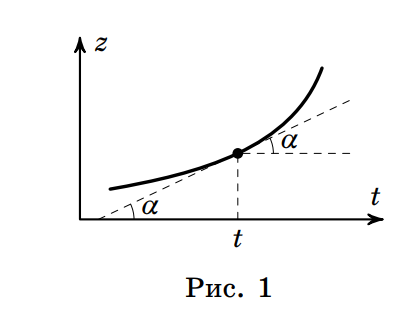
\includegraphics[width=0.25\textwidth]{g.png}
\end{wrapfigure}
означает, что функция \( f \) либо возрастающая (если \( t' < t'' \), то \( f(t') < f(t'') \)), либо убывающая (если \( t' < t'' \), то \( f(t') > f(t'') \)). Будем для определённости считать функцию \( f \) возрастающей. Тогда множество значений функции \( f \) на отрезке \( [t_1, t_2] \) представляет собой отрезок \( [z_1, z_2] \), где \( z_1 = f(t_1) \), \( z_2 = f(t_2) \) (рис. 2). 

\end{document}
